\documentclass{article}
\usepackage[english]{babel}
\usepackage{longtable}
\usepackage[top=1in, bottom=0.25in, left=1.25in, right=1.25in,includefoot,heightrounded]{geometry}
\usepackage{indentfirst}
\usepackage[utf8]{inputenc}
\usepackage{amsmath,amssymb}
\usepackage{graphicx,tikz}
\usepackage{hyperref}
\usepackage[colorinlistoftodos]{todonotes}
\usepackage[document]{ragged2e}
\usepackage{fancyhdr}
\usepackage{enumerate}
\usepackage{listings}
\usepackage{color}
\usepackage{flowchart}
\usepackage{hyperref}
\usetikzlibrary{arrows}

\usetikzlibrary{shapes.geometric, arrows}
\tikzstyle{startstop} = [rectangle, rounded corners, minimum width=3cm, minimum height=1cm,text centered, draw=black, fill=red!30]
\tikzstyle{decision} = [diamond, minimum width=4cm, minimum height=0.5cm, text centered, draw=black, fill=green!30]
\tikzstyle{process} = [rectangle, minimum width=3cm, minimum height=1cm, text centered, draw=black, fill=orange!30]
\tikzstyle{arrow} = [thick,->,>=stealth]
\tikzstyle{io} = [trapezium, trapezium left angle=70, trapezium right angle=110, minimum width=2cm, text width=4cm, minimum height=1cm, text centered, draw=black, fill=blue!30]

\pagestyle{fancy}
\fancyhf{}
\lhead{Myles Deslippe}
\rhead{Comp 3300 | Operating System Fundamentals}
\cfoot{\thepage}

\definecolor{MyDarkGreen}{rgb}{0.0,0.4,0.0}
\lstset{inputencoding=ansinew}
\lstset{breaklines=true} 

\begin{document}

    \section*{\centering{Main Memory}}

    \subsection*{Background Information}
    \begin{itemize}
        \item A \textbf{program} must be \textbf{read into memory} from \textbf{secondary storage} (for example a disk) and placed within a \textbf{process} inorder to allow the program to \textbf{execute}.
        \item \textbf{Main memory} and \textbf{registers} are storage that is \textbf{directly accessable by the CPU only}.
        \item \textbf{Register access} only required a maximum of \textbf{one CPU clock cycle}.
        \item \textbf{Main memory} can take \textbf{several clock cycles}, and may cause a stall.
        \item To prevent the \textbf{main memory from stalling}, we use \textbf{cache}; cache sits inbetween the main memory, and the registers.
        \item \textbf{Protection} may be required to \textbf{ensure correct operation} (for example if a processor has two or more cores which share a single cache).
    \end{itemize}

    \subsection*{Base and Limit Registers}
    \begin{itemize}
        \item A \textbf{pair of base and limit registers} are used to define the \textbf{logical address space} for a process.
        \item The \textbf{CPU} must check every \textbf{memory access generated} in \textbf{user mode} to ensure it is within the \textbf{users base and limit}.
        \item[] \includegraphics*[width=\textwidth - 25pt]{images/Base-Limit.PNG}
    \end{itemize}

    \subsection*{Address Binding}
    \begin{itemize}
        \item \textbf{Addresses} are represented in \textbf{different ways} at \textbf{different stages} of a \textbf{program's life}.
        \begin{itemize}
            \item \textbf{Source code addresses} typically contain a \textbf{symbolic reference} (eg variables).
            \item \textbf{Compiled code addresses} bind to \textbf{relocatable addresses} (eg 14 bytes after the start of this module).
            \item The \textbf{linker} or \textbf{loader} will \textbf{bind relocatable addreses} to \textbf{absolute adresses} (the actual address, not an offset).
        \end{itemize}
        \item \textbf{Address binding} of \textbf{instructions and data} to \textbf{memory addresses} can happen a three different stages:
        \begin{enumerate}
            \item \textbf{Compile Time} | If the memory location is known prior, absolute code can be generated. This is not optomal, as it needs to be recompiled if the address changes.
            \item \textbf{Load Time} | Final binding is delayed until load time. If the starting address changes, we only reload the user code to incorporate this changed value.
            \item \textbf{Execution Time} | Binding is delayed until runtime. This is done if the process can be moved during it's execution from one memory segment to another. This requires hardware support for address maps (eg base and limit registers).
        \end{enumerate}
    \end{itemize}

    \subsection*{Static vs Dynamic Linking}
    \begin{itemize}
        \item \textbf{Static linking} is when the \textbf{code} for all \textbf{routines} called by your program become \textbf{a part of the executable file}. 
        \item \textbf{Dynamic linking} is when the \textbf{code} for some \textbf{external routines} are \textbf{located when the program runs}.
        \begin{itemize}
            \item \textbf{Dynamic linking} is useful for \textbf{shared libraries}.
        \end{itemize}
        \item With \textbf{dynamic linking}, a \textbf{code stub} is used to \textbf{locate the appropriate memory-resident library routine}. The stub is replaced with the address of the routine, and executes the routine.
        \item If a \textbf{routine} that is being \textbf{dynamically linked} is not in the \textbf{process' address space} the operating system will \textbf{add it} to the address space.
        \item Not all operating systems support dynamic linking.
    \end{itemize}

    \subsection*{Logical vs Physical Address Space}
    \begin{itemize}
        \item The concept that \textbf{logical address space} is bound to \textbf{physical address space}, is essential for \textbf{proper memory managment}.
        \item \textbf{Logical Addresses} are addresses that are \textbf{generated by the CPU} (also know as virtual addresses).
        \item \textbf{Physical Adresses} are adresses that are \textbf{managed by the memory unit}.
        \item \textbf{Logical (virtual)} and \textbf{physical} addresses have a different \textbf{execution-time address-binding} scheme.
    \end{itemize}

    \subsection*{Memory-Management Unit (MMU)}
    \begin{itemize}
        \item A \textbf{Memory-Management Unit (MMU)} is a \textbf{hardware device} that \textbf{maps virtual addresses to physical adresses} at \textbf{runtime}.
        \item[] \includegraphics*[width=\textwidth - 25pt]{images/Memory-Managment-Unit.PNG}
        \item A \textbf{partition table} is used to store the \textbf{allocated, and available physical memory}. Along with the \textbf{process id} of \textbf{memory that is allocated}.
        \item The \textbf{dynamic storage-allocation problem} refers to the problem that arises when we need to dynamically allocate memory in a partation table. The following algorithms can be used:
        \begin{enumerate}
            \item \textbf{First-Fit} | Allocate the first hole that is big enough.
            \item \textbf{Best-Fit} | Allocate the smallest hole that is big enough; must search the entire table, unless the table is ordered by size.
            \item \textbf{Worst-Fit} | Allocate the largest hole; must search the entire table, unless the table is sorted.
        \end{enumerate}
        \begin{itemize}
            \item Best fit is slower than first fit, but more efficient with memory use.
        \end{itemize}
    \end{itemize}

    \subsection*{Memory Fragmentation}
    \begin{itemize}
        \item \textbf{External fragmentation} occurs when the \textbf{total memory space exists} to satisfy a request, but the \textbf{memory space is not contiguous}.
        \begin{itemize}
            \item The memory is said to be \textbf{fragmented} (broken into seperate parts).
        \end{itemize}
        \item To \textbf{fix fragmentation} we use \textbf{compaction}; a very \textbf{expensive operation}.
        \item \textbf{Compaction} consists of \textbf{shuffling memory contents} to place \textbf{all free memory together} in one large block.
        \item \textbf{Compaction} is only possible if \textbf{relocation is dynamic}, and done at \textbf{execution time}.
        \item First-Fit, Best-Fit, and Worst-Fit all \textbf{cause fragmentation}.
        \item Modern operating systems instead use \textbf{virtual memory} and \textbf{segmentation} to manage memory, avoiding fragmentation.
    \end{itemize}

    \subsection*{Virtual Memory}
    \begin{itemize}
        \item \textbf{Virtual memory} is acheived by \textbf{splitting the main memory} into \textbf{fixed-size partitions} known as \textbf{page frames}.
        \item \textbf{Page frames are typically 4KB}.
        \item \textbf{Processes} are then split into \textbf{blocks of equal size} (block size = page frame size).
        \begin{itemize}
            \item The blocks do not have to be contiguous.
        \end{itemize}
        \item A page table is then used to map each \textbf{block} in \textbf{virtual memory} to a distinct \textbf{page} in \textbf{physical memory}.
        \item This \textbf{removes} of \textbf{fragmentation}, as each virtual memory block appears to be \textbf{contiguous} to the CPU.
        \item When using \textbf{virtual memory}, you \textbf{do not need to load all of the program} into memory at the \textbf{start}, they can be loaded later on.
        \begin{itemize}
            \item This is known as \textbf{demand paging}; pages are \textbf{loaded into the main memory} when they are first used.
            \item If the \textbf{primary memory is full} when a \textbf{page} needs to be \textbf{loaded}, the operation system will perform a \textbf{swap}; the operating system will save a block already in ram, load the one currently needed, and when it is done the original one will be place back into memory. \textbf{Secondary memory} usually has a \textbf{swap partition} for this scenerio.
            \item There are different swap replacement policies: first in first out, least recently used, least frequently used, etc. 
        \end{itemize}
    \end{itemize}

    \subsection*{Shared Paging}
    \begin{itemize}
        \item \textbf{Common library routines} can be shared throughout \textbf{all processes} running on the operating system.
        \item This can be acheived with \textbf{shared pages}.
    \end{itemize}

    \subsection*{Copy on Write (COW)}
    \begin{itemize}
        \item All \textbf{parent pages} are initallly marked as \textbf{shared}.
        \item When \textbf{data} in any of the \textbf{shared pages change} (by the parent or any child), the \textbf{OS intercepts} and makes a \textbf{copy of the change}.
        \item The \textbf{parent and all children} will have the \textbf{same copy of unmodified pages}.
        \item This is done to save memory.
    \end{itemize}

    \subsection*{Address Translation Scheme}
    \begin{abstract}
        \item The \textbf{page table} consits of four columns: block, page frame, present bit, dirty bit.
        \item The \textbf{page table} has a \textbf{page-table base register (PTBR)}.
        \item Each \textbf{virtual address} is composed of \textbf{a page number, and an offset}.
        \item The page number refers to the virtual page number, and the offset is the number of bytes from the start of the page that the data resides.
        \item On \textbf{32-bit systems} the \textbf{maximum process size is 4GB} ($2^{32}$).
    \end{abstract}

    \subsection*{Hierarchical Page Tables}
    \begin{itemize}
        \item \textbf{Hierarchical page tables} divide addresses into three sections:
        \begin{enumerate}
            \item \textbf{The directory (Dir)} | First 10 bits.
            \item \textbf{The Table} | Next 10 bits.
            \item \textbf{The Offset} | Last 12 bits.
        \end{enumerate}
        \item The directory refers to a table that references other page tables. The table section of the address refers to the index of the referenced page table that we are interested in, the offset is the number of bytes from the start of the of the page.
        \item[] 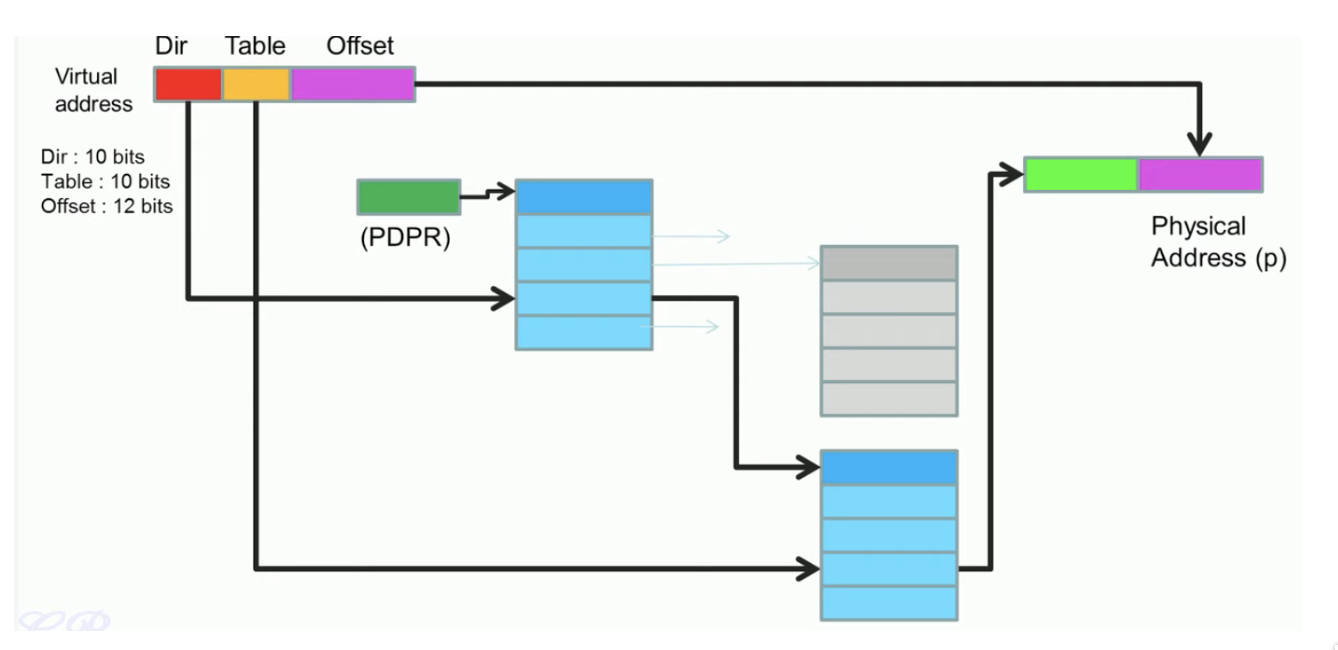
\includegraphics[width=\textwidth - 25pt]{images/Hierarchial-Page-Table.png}
        \item \textbf{Hierarchical page tables} allow us to store page tables in memory that is \textbf{not contiguous}. As page tables can get very large (32-bit systems need a 4MB page table per process). 
        \item You can continue to add \textbf{more levels} to the hierachy for systems with more memory (eg 64-bit).
    \end{itemize}

    \subsection*{Hash Page Tables}
    \begin{itemize}
        \item An efficient way to \textbf{map addresses} is with \textbf{hashed page tables}.
        \item You use a hashtable with a linkedlist to map values to adresses.
        \item[] 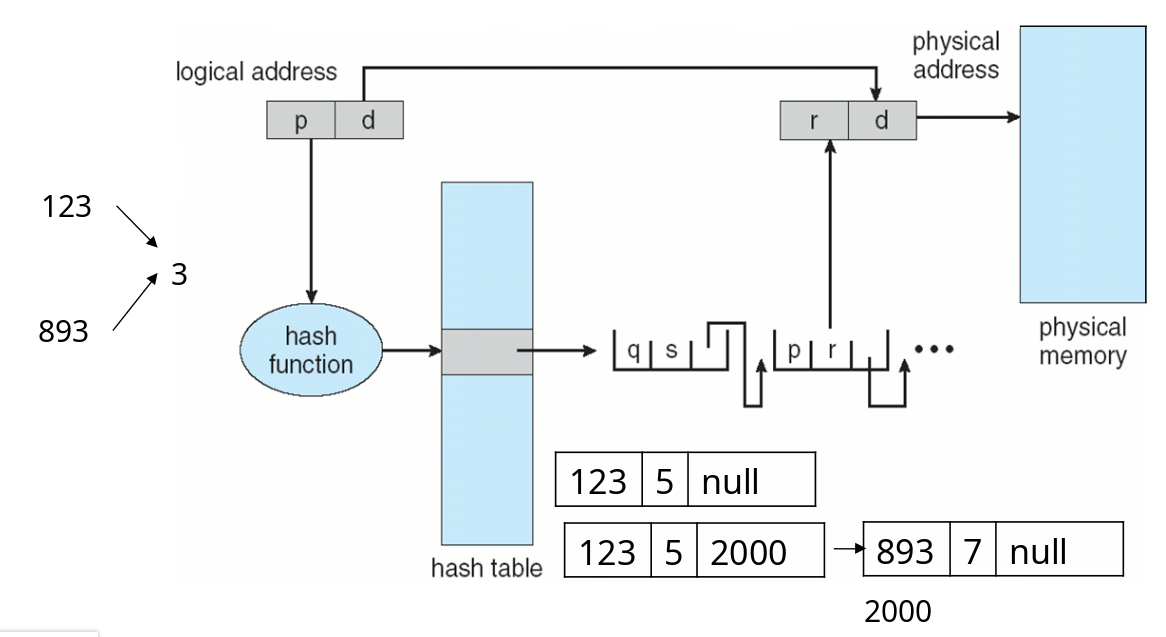
\includegraphics[width=\textwidth - 25pt]{images/Hash-Page-Table.png}
    \end{itemize}

    \subsection*{Inverted Page Tables}
    \begin{itemize}
        \item A \textbf{modern} way to implement page tables is with \textbf{inverted page tables}.
        \item An \textbf{Inverted page table} is a page table that is shared with \textbf{all processes}, with addresses composed of process id's, block number, and offset.
        \item This \textbf{solves the problem} of \textbf{wasting a lot of memory} creating \textbf{page tables} for each process.
        \item[] 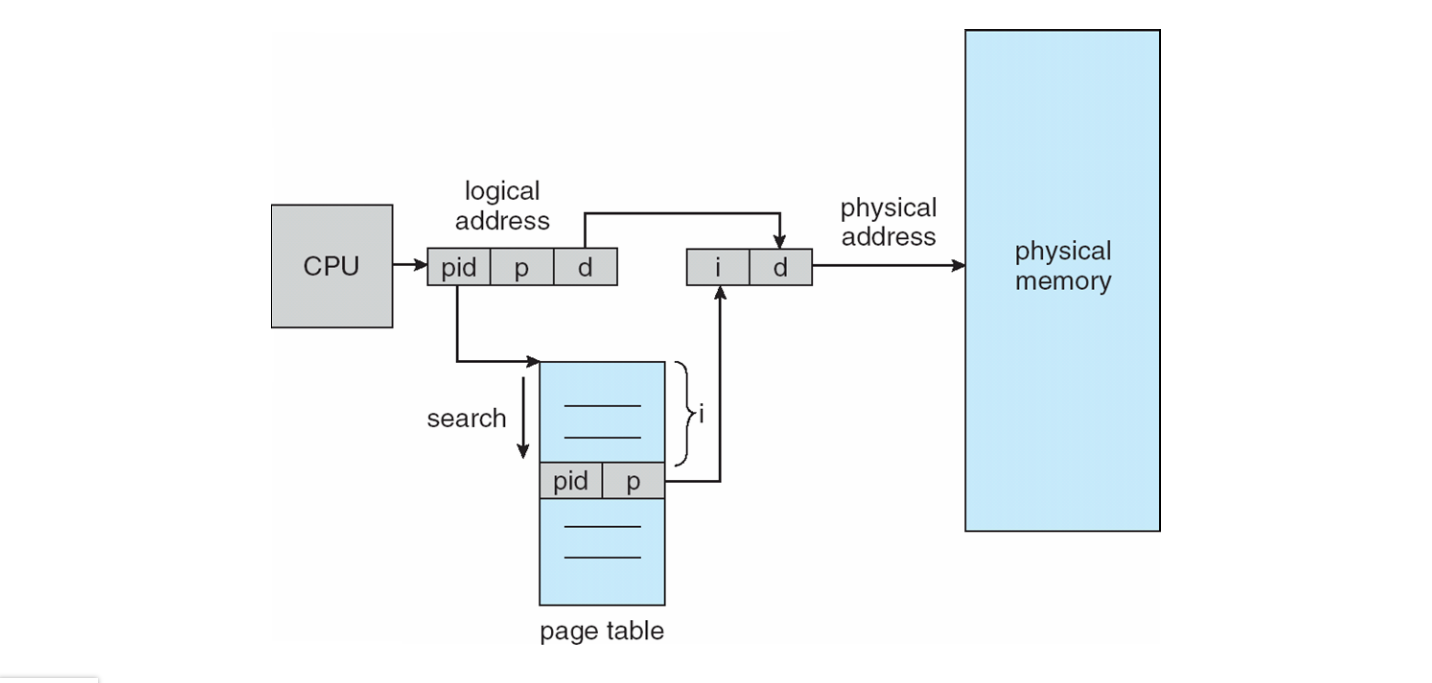
\includegraphics[width=\textwidth - 25pt]{images/Inverted-Page-Table.png}
    \end{itemize}

\end{document}
